\documentclass[main.tex]{subfiles}

\begin{document}\pagestyle{empty}

%─────────────────────────────
% 1. STRANA – titulní s celostránkovou fotkou
%─────────────────────────────
\clearpage
\thispagestyle{empty}

% Celostránková fotka na pozadí (nahraď placeholder.jpg skutečným souborem)
\AddToShipoutPictureBG*{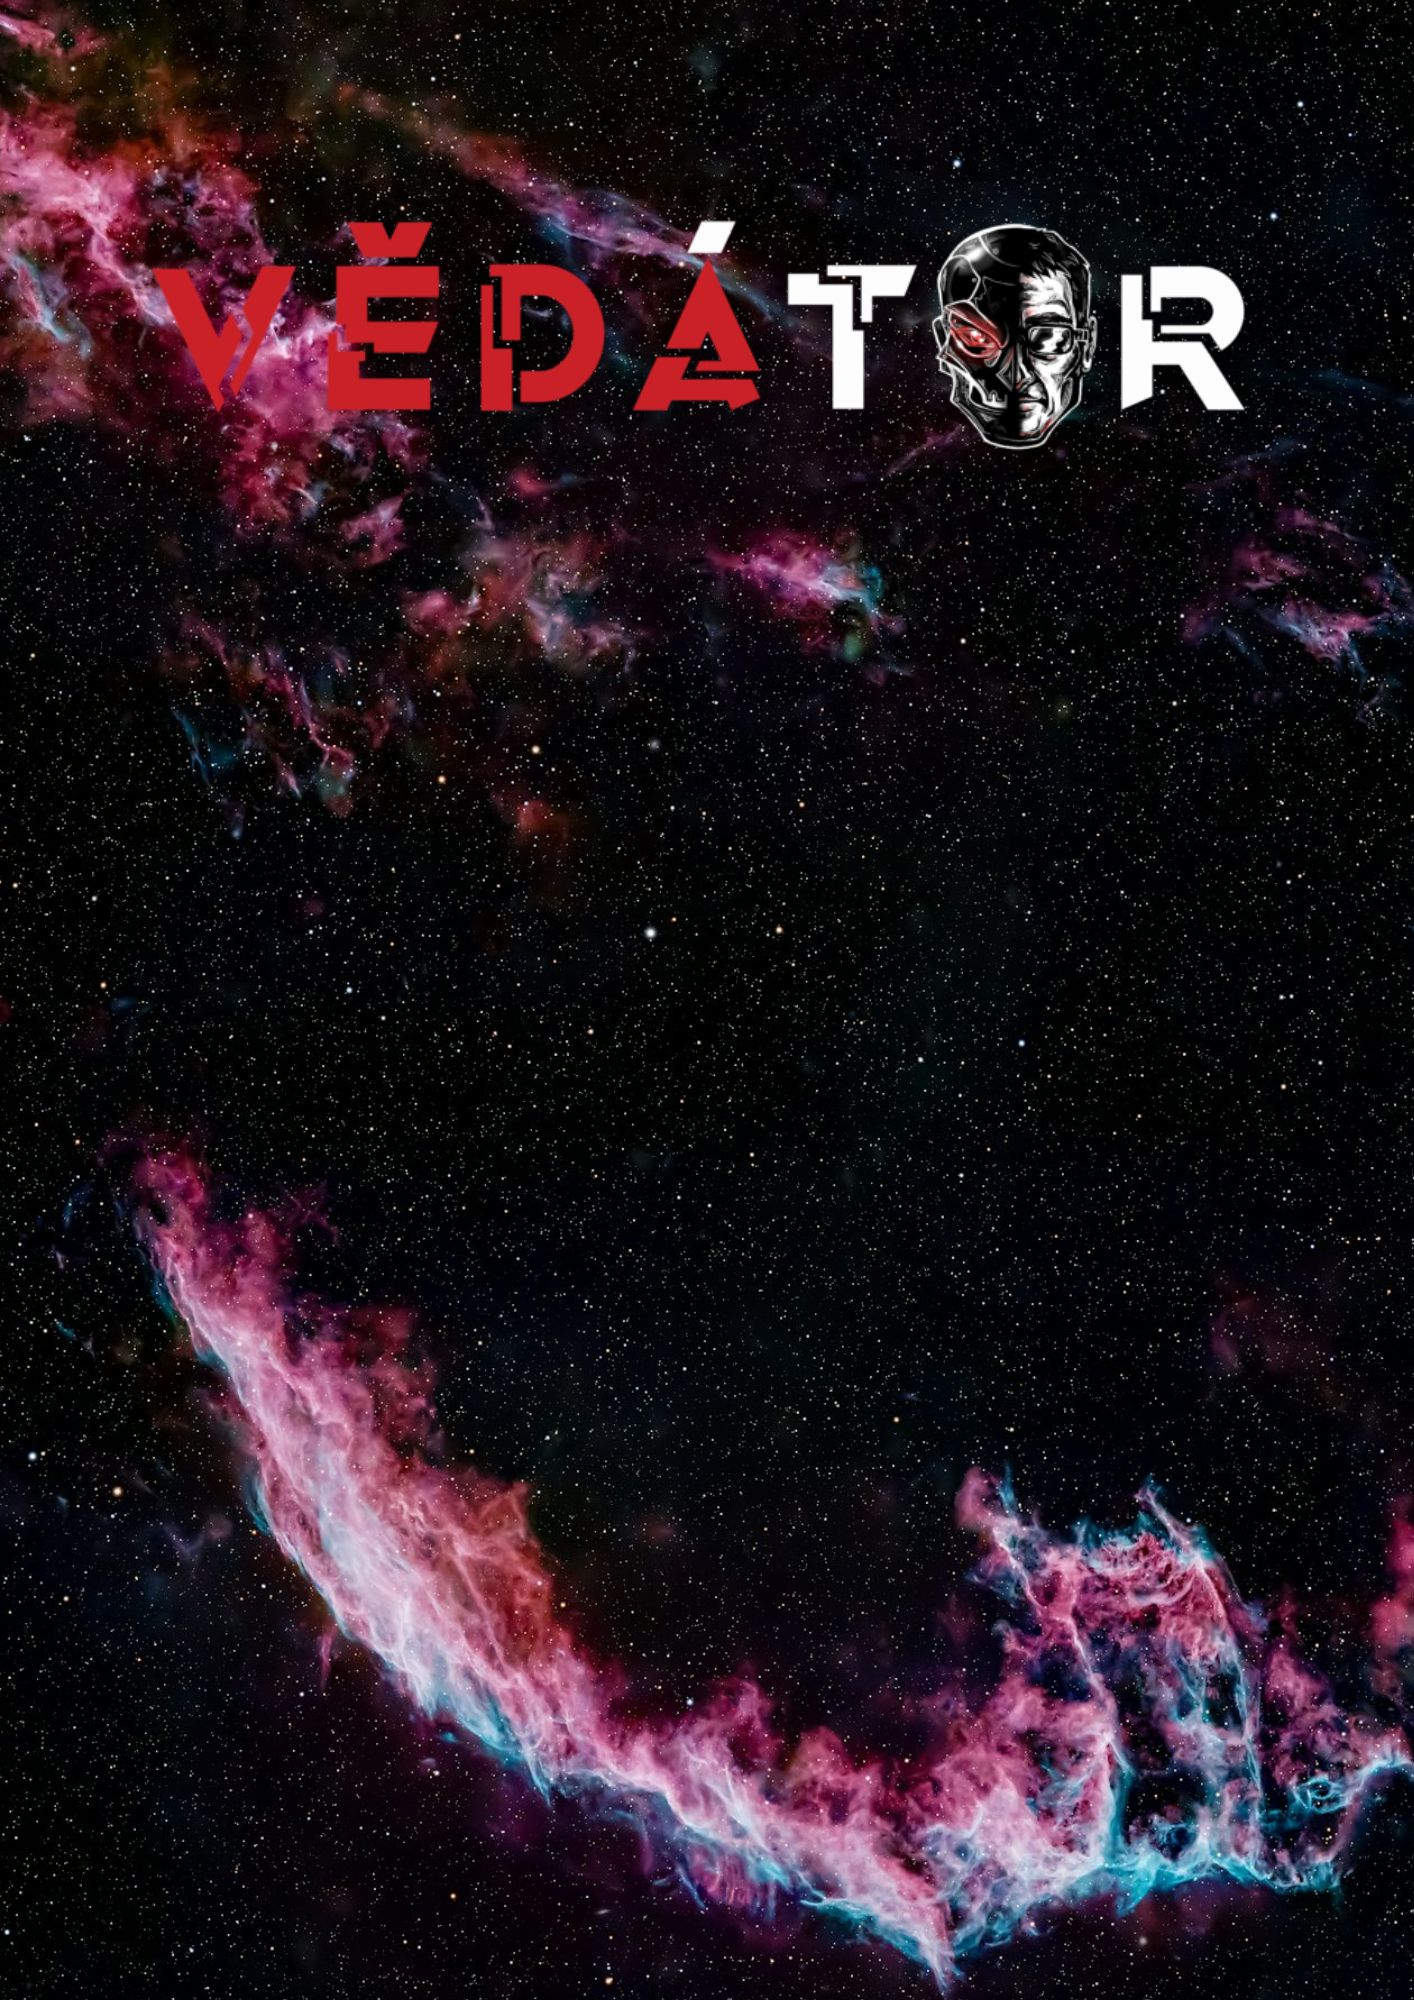
\includegraphics[width=\paperwidth,height=\paperheight]{frontmatter}};

\vspace*{0.62\textheight}   % posune text do spodní třetiny (můžeš doladit)

\begin{center}
    \color{white}\Huge\bfseries\sffamily
    \docname\par
    \vspace{2em}
    \color{white}\LARGE
    \docauth
\end{center}

\clearpage

%─────────────────────────────
% 2. STRANA – tiráž / impressum (pravý dolní roh)
%─────────────────────────────
\clearpage
\thispagestyle{empty}

\vspace*{\fill}    % odtlačí vše dolů

\hfill\begin{minipage}{0.6\textwidth}
\raggedleft               % zarovná text uvnitř minipage doprava
\parindent=0pt            % žádné odsazení odstavců (v tiráži to vypadá lépe)

{\footnotesize
Šéfredaktor projektu a hlavní autor textů: \textbf{Bc. Ladislav Loukota} (1993).\\
Vystudoval žurnalistiku a anglistiku na Filozofické fakultě Univerzity Palackého v Olomouci.
Je zakladatelem a šéfredaktorem nezávislého popularizačního serveru Vědátor (od roku 2016).
Pracuje jako PR specialista Ústavu organické chemie a biochemie AV ČR.

\bigskip
Autoři textů: \textbf{Bc. Ladislav Loukota} a \textbf{Filip Šlapal, LL}.

\bigskip
Autor fotografií a ilustrací: Kolektiv Vědátoru a veřejně dostupné zdroje.

\bigskip
Články původně vyšly na populárně-naučném serveru \emph{Vědátor.org} v období prosinec 2025 – únor 2026.\\
Pro toto tištěné vydání byly převzaty v plném znění a upraveny pouze formálně (odstraněny některé internetové meme obrázky, které se nevešly na stránku).

\bigskip
\nocite{sliz}
\nocite{spalnicky}
\nocite{sars}
\nocite{overthink}
\nocite{lava}
\nocite{mysl}
\nocite{fialova}
\nocite{hudba}
\nocite{sklo}
\nocite{sinaj}

\printbibliography[heading=none]
}

\end{minipage}

\clearpage

%─────────────────────────────
% 3. STRANA – obsah
%─────────────────────────────
\thispagestyle{empty}

% Přejmenujeme obsah na „Obsah“ a dáme stejný font jako kapitoly
\renewcommand{\contentsname}{Obsah}
\tableofcontents

\thispagestyle{empty}
\clearpage
\thispagestyle{empty}
\end{document}